% Created by tikzDevice version GitHub Dev on 2012-08-10 11:55:09
% !TEX encoding = UTF-8 Unicode
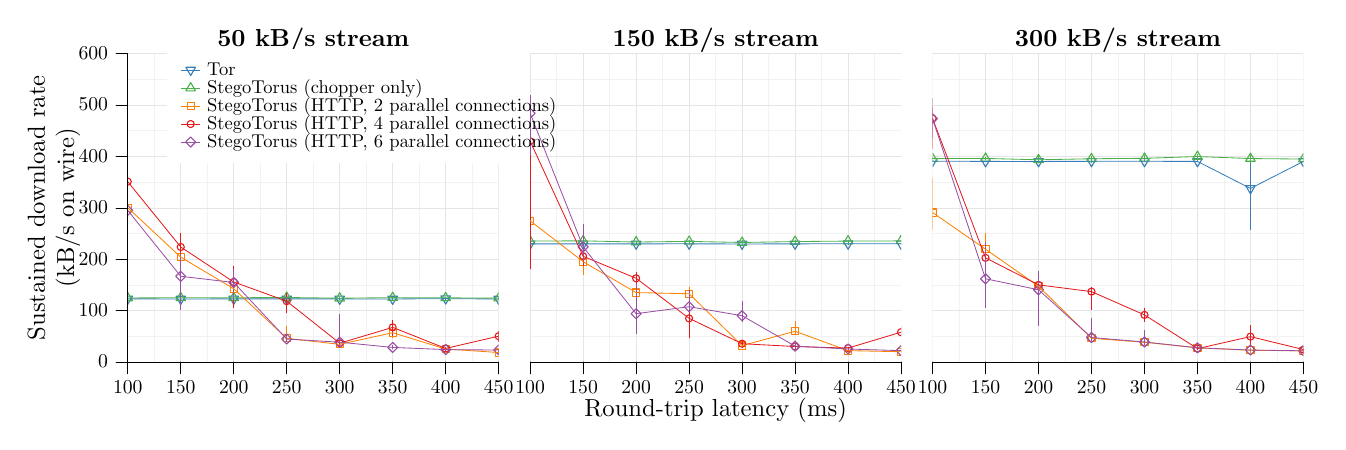
\begin{tikzpicture}[x=1pt,y=1pt]
\definecolor[named]{fillColor}{rgb}{1.00,1.00,1.00}
\begin{scope}
\path[clip] ( 38.09, 22.25) rectangle (172.12,133.66);
\definecolor[named]{drawColor}{rgb}{0.95,0.95,0.95}

\path[draw=drawColor,line width= 0.2pt,line join=round,line cap=round] ( 38.09, 31.54) --
	(172.12, 31.54);

\path[draw=drawColor,line width= 0.2pt,line join=round,line cap=round] ( 38.09, 50.11) --
	(172.12, 50.11);

\path[draw=drawColor,line width= 0.2pt,line join=round,line cap=round] ( 38.09, 68.67) --
	(172.12, 68.67);

\path[draw=drawColor,line width= 0.2pt,line join=round,line cap=round] ( 38.09, 87.24) --
	(172.12, 87.24);

\path[draw=drawColor,line width= 0.2pt,line join=round,line cap=round] ( 38.09,105.81) --
	(172.12,105.81);

\path[draw=drawColor,line width= 0.2pt,line join=round,line cap=round] ( 38.09,124.38) --
	(172.12,124.38);

\path[draw=drawColor,line width= 0.2pt,line join=round,line cap=round] ( 47.67, 22.25) --
	( 47.67,133.66);

\path[draw=drawColor,line width= 0.2pt,line join=round,line cap=round] ( 66.81, 22.25) --
	( 66.81,133.66);

\path[draw=drawColor,line width= 0.2pt,line join=round,line cap=round] ( 85.96, 22.25) --
	( 85.96,133.66);

\path[draw=drawColor,line width= 0.2pt,line join=round,line cap=round] (105.11, 22.25) --
	(105.11,133.66);

\path[draw=drawColor,line width= 0.2pt,line join=round,line cap=round] (124.25, 22.25) --
	(124.25,133.66);

\path[draw=drawColor,line width= 0.2pt,line join=round,line cap=round] (143.40, 22.25) --
	(143.40,133.66);

\path[draw=drawColor,line width= 0.2pt,line join=round,line cap=round] (162.54, 22.25) --
	(162.54,133.66);
\definecolor[named]{drawColor}{rgb}{0.90,0.90,0.90}

\path[draw=drawColor,line width= 0.2pt,line join=round,line cap=round] ( 38.09, 22.25) --
	(172.12, 22.25);

\path[draw=drawColor,line width= 0.2pt,line join=round,line cap=round] ( 38.09, 40.82) --
	(172.12, 40.82);

\path[draw=drawColor,line width= 0.2pt,line join=round,line cap=round] ( 38.09, 59.39) --
	(172.12, 59.39);

\path[draw=drawColor,line width= 0.2pt,line join=round,line cap=round] ( 38.09, 77.96) --
	(172.12, 77.96);

\path[draw=drawColor,line width= 0.2pt,line join=round,line cap=round] ( 38.09, 96.53) --
	(172.12, 96.53);

\path[draw=drawColor,line width= 0.2pt,line join=round,line cap=round] ( 38.09,115.10) --
	(172.12,115.10);

\path[draw=drawColor,line width= 0.2pt,line join=round,line cap=round] ( 38.09,133.66) --
	(172.12,133.66);

\path[draw=drawColor,line width= 0.2pt,line join=round,line cap=round] ( 38.09, 22.25) --
	( 38.09,133.66);

\path[draw=drawColor,line width= 0.2pt,line join=round,line cap=round] ( 57.24, 22.25) --
	( 57.24,133.66);

\path[draw=drawColor,line width= 0.2pt,line join=round,line cap=round] ( 76.39, 22.25) --
	( 76.39,133.66);

\path[draw=drawColor,line width= 0.2pt,line join=round,line cap=round] ( 95.53, 22.25) --
	( 95.53,133.66);

\path[draw=drawColor,line width= 0.2pt,line join=round,line cap=round] (114.68, 22.25) --
	(114.68,133.66);

\path[draw=drawColor,line width= 0.2pt,line join=round,line cap=round] (133.82, 22.25) --
	(133.82,133.66);

\path[draw=drawColor,line width= 0.2pt,line join=round,line cap=round] (152.97, 22.25) --
	(152.97,133.66);

\path[draw=drawColor,line width= 0.2pt,line join=round,line cap=round] (172.12, 22.25) --
	(172.12,133.66);
\definecolor[named]{drawColor}{rgb}{0.22,0.49,0.72}

\path[draw=drawColor,line width= 0.3pt,line join=round] ( 38.09, 44.80) -- ( 38.09, 45.15);

\path[draw=drawColor,line width= 0.3pt,line join=round] ( 57.24, 44.92) -- ( 57.24, 45.20);

\path[draw=drawColor,line width= 0.3pt,line join=round] ( 76.39, 45.05) -- ( 76.39, 45.10);

\path[draw=drawColor,line width= 0.3pt,line join=round] ( 95.53, 45.00) -- ( 95.53, 45.10);

\path[draw=drawColor,line width= 0.3pt,line join=round] (114.68, 45.01) -- (114.68, 45.13);

\path[draw=drawColor,line width= 0.3pt,line join=round] (133.82, 44.98) -- (133.82, 45.10);

\path[draw=drawColor,line width= 0.3pt,line join=round] (152.97, 44.86) -- (152.97, 45.14);

\path[draw=drawColor,line width= 0.3pt,line join=round] (172.12, 44.89) -- (172.12, 45.18);

\path[draw=drawColor,line width= 0.4pt,line join=round,line cap=round] ( 38.09, 43.07) --
	( 39.82, 46.05) --
	( 36.37, 46.05) --
	( 38.09, 43.07);

\path[draw=drawColor,line width= 0.4pt,line join=round,line cap=round] ( 57.24, 43.02) --
	( 58.96, 46.00) --
	( 55.52, 46.00) --
	( 57.24, 43.02);

\path[draw=drawColor,line width= 0.4pt,line join=round,line cap=round] ( 76.39, 43.05) --
	( 78.11, 46.04) --
	( 74.66, 46.04) --
	( 76.39, 43.05);

\path[draw=drawColor,line width= 0.4pt,line join=round,line cap=round] ( 95.53, 43.07) --
	( 97.26, 46.05) --
	( 93.81, 46.05) --
	( 95.53, 43.07);

\path[draw=drawColor,line width= 0.4pt,line join=round,line cap=round] (114.68, 43.05) --
	(116.40, 46.03) --
	(112.95, 46.03) --
	(114.68, 43.05);

\path[draw=drawColor,line width= 0.4pt,line join=round,line cap=round] (133.82, 43.02) --
	(135.55, 46.01) --
	(132.10, 46.01) --
	(133.82, 43.02);

\path[draw=drawColor,line width= 0.4pt,line join=round,line cap=round] (152.97, 43.14) --
	(154.70, 46.13) --
	(151.25, 46.13) --
	(152.97, 43.14);

\path[draw=drawColor,line width= 0.4pt,line join=round,line cap=round] (172.12, 43.01) --
	(173.84, 46.00) --
	(170.39, 46.00) --
	(172.12, 43.01);
\definecolor[named]{drawColor}{rgb}{0.30,0.69,0.29}

\path[draw=drawColor,line width= 0.3pt,line join=round] ( 38.09, 44.95) -- ( 38.09, 45.74);

\path[draw=drawColor,line width= 0.3pt,line join=round] ( 57.24, 45.32) -- ( 57.24, 45.70);

\path[draw=drawColor,line width= 0.3pt,line join=round] ( 76.39, 45.06) -- ( 76.39, 45.66);

\path[draw=drawColor,line width= 0.3pt,line join=round] ( 95.53, 45.17) -- ( 95.53, 45.66);

\path[draw=drawColor,line width= 0.3pt,line join=round] (114.68, 45.03) -- (114.68, 45.82);

\path[draw=drawColor,line width= 0.3pt,line join=round] (133.82, 44.90) -- (133.82, 45.70);

\path[draw=drawColor,line width= 0.3pt,line join=round] (152.97, 45.04) -- (152.97, 45.74);

\path[draw=drawColor,line width= 0.3pt,line join=round] (172.12, 45.04) -- (172.12, 45.65);

\path[draw=drawColor,line width= 0.4pt,line join=round,line cap=round] ( 38.09, 47.37) --
	( 39.82, 44.38) --
	( 36.37, 44.38) --
	( 38.09, 47.37);

\path[draw=drawColor,line width= 0.4pt,line join=round,line cap=round] ( 57.24, 47.44) --
	( 58.96, 44.46) --
	( 55.52, 44.46) --
	( 57.24, 47.44);

\path[draw=drawColor,line width= 0.4pt,line join=round,line cap=round] ( 76.39, 47.44) --
	( 78.11, 44.46) --
	( 74.66, 44.46) --
	( 76.39, 47.44);

\path[draw=drawColor,line width= 0.4pt,line join=round,line cap=round] ( 95.53, 47.54) --
	( 97.26, 44.55) --
	( 93.81, 44.55) --
	( 95.53, 47.54);

\path[draw=drawColor,line width= 0.4pt,line join=round,line cap=round] (114.68, 47.28) --
	(116.40, 44.29) --
	(112.95, 44.29) --
	(114.68, 47.28);

\path[draw=drawColor,line width= 0.4pt,line join=round,line cap=round] (133.82, 47.48) --
	(135.55, 44.49) --
	(132.10, 44.49) --
	(133.82, 47.48);

\path[draw=drawColor,line width= 0.4pt,line join=round,line cap=round] (152.97, 47.42) --
	(154.70, 44.44) --
	(151.25, 44.44) --
	(152.97, 47.42);

\path[draw=drawColor,line width= 0.4pt,line join=round,line cap=round] (172.12, 47.29) --
	(173.84, 44.30) --
	(170.39, 44.30) --
	(172.12, 47.29);
\definecolor[named]{drawColor}{rgb}{1.00,0.50,0.00}

\path[draw=drawColor,line width= 0.3pt,line join=round] ( 38.09, 63.49) -- ( 38.09, 95.04);

\path[draw=drawColor,line width= 0.3pt,line join=round] ( 57.24, 57.62) -- ( 57.24, 63.51);

\path[draw=drawColor,line width= 0.3pt,line join=round] ( 76.39, 46.69) -- ( 76.39, 52.70);

\path[draw=drawColor,line width= 0.3pt,line join=round] ( 95.53, 29.71) -- ( 95.53, 35.32);

\path[draw=drawColor,line width= 0.3pt,line join=round] (114.68, 28.31) -- (114.68, 29.79);

\path[draw=drawColor,line width= 0.3pt,line join=round] (133.82, 30.89) -- (133.82, 36.36);

\path[draw=drawColor,line width= 0.3pt,line join=round] (152.97, 26.24) -- (152.97, 27.43);

\path[draw=drawColor,line width= 0.3pt,line join=round] (172.12, 24.69) -- (172.12, 26.66);

\path[draw=drawColor,line width= 0.4pt,line join=round,line cap=round] ( 36.81, 76.71) rectangle ( 39.37, 79.27);

\path[draw=drawColor,line width= 0.4pt,line join=round,line cap=round] ( 55.96, 58.85) rectangle ( 58.52, 61.41);

\path[draw=drawColor,line width= 0.4pt,line join=round,line cap=round] ( 75.11, 47.43) rectangle ( 77.67, 49.99);

\path[draw=drawColor,line width= 0.4pt,line join=round,line cap=round] ( 94.25, 29.51) rectangle ( 96.81, 32.07);

\path[draw=drawColor,line width= 0.4pt,line join=round,line cap=round] (113.40, 27.34) rectangle (115.96, 29.90);

\path[draw=drawColor,line width= 0.4pt,line join=round,line cap=round] (132.54, 31.53) rectangle (135.10, 34.10);

\path[draw=drawColor,line width= 0.4pt,line join=round,line cap=round] (151.69, 25.66) rectangle (154.25, 28.22);

\path[draw=drawColor,line width= 0.4pt,line join=round,line cap=round] (170.84, 24.38) rectangle (173.40, 26.94);
\definecolor[named]{drawColor}{rgb}{0.89,0.10,0.11}

\path[draw=drawColor,line width= 0.3pt,line join=round] ( 38.09, 68.00) -- ( 38.09,104.32);

\path[draw=drawColor,line width= 0.3pt,line join=round] ( 57.24, 57.19) -- ( 57.24, 68.82);

\path[draw=drawColor,line width= 0.3pt,line join=round] ( 76.39, 41.83) -- ( 76.39, 56.80);

\path[draw=drawColor,line width= 0.3pt,line join=round] ( 95.53, 39.84) -- ( 95.53, 47.33);

\path[draw=drawColor,line width= 0.3pt,line join=round] (114.68, 27.62) -- (114.68, 30.08);

\path[draw=drawColor,line width= 0.3pt,line join=round] (133.82, 31.80) -- (133.82, 37.48);

\path[draw=drawColor,line width= 0.3pt,line join=round] (152.97, 26.45) -- (152.97, 27.50);

\path[draw=drawColor,line width= 0.3pt,line join=round] (172.12, 29.50) -- (172.12, 33.32);

\path[draw=drawColor,line width= 0.4pt,line join=round,line cap=round] ( 38.09, 87.40) circle (  1.28);

\path[draw=drawColor,line width= 0.4pt,line join=round,line cap=round] ( 57.24, 63.79) circle (  1.28);

\path[draw=drawColor,line width= 0.4pt,line join=round,line cap=round] ( 76.39, 51.15) circle (  1.28);

\path[draw=drawColor,line width= 0.4pt,line join=round,line cap=round] ( 95.53, 44.21) circle (  1.28);

\path[draw=drawColor,line width= 0.4pt,line join=round,line cap=round] (114.68, 29.02) circle (  1.28);

\path[draw=drawColor,line width= 0.4pt,line join=round,line cap=round] (133.82, 34.75) circle (  1.28);

\path[draw=drawColor,line width= 0.4pt,line join=round,line cap=round] (152.97, 27.14) circle (  1.28);

\path[draw=drawColor,line width= 0.4pt,line join=round,line cap=round] (172.12, 31.58) circle (  1.28);
\definecolor[named]{drawColor}{rgb}{0.60,0.31,0.64}

\path[draw=drawColor,line width= 0.3pt,line join=round] ( 38.09, 64.78) -- ( 38.09,105.02);

\path[draw=drawColor,line width= 0.3pt,line join=round] ( 57.24, 41.09) -- ( 57.24, 61.38);

\path[draw=drawColor,line width= 0.3pt,line join=round] ( 76.39, 44.95) -- ( 76.39, 55.95);

\path[draw=drawColor,line width= 0.3pt,line join=round] ( 95.53, 29.48) -- ( 95.53, 32.21);

\path[draw=drawColor,line width= 0.3pt,line join=round] (114.68, 28.49) -- (114.68, 39.75);

\path[draw=drawColor,line width= 0.3pt,line join=round] (133.82, 26.77) -- (133.82, 28.35);

\path[draw=drawColor,line width= 0.3pt,line join=round] (152.97, 26.39) -- (152.97, 27.51);

\path[draw=drawColor,line width= 0.3pt,line join=round] (172.12, 25.24) -- (172.12, 27.04);

\path[draw=drawColor,line width= 0.4pt,line join=round,line cap=round] ( 36.28, 77.01) --
	( 38.09, 78.82) --
	( 39.90, 77.01) --
	( 38.09, 75.20) --
	( 36.28, 77.01);

\path[draw=drawColor,line width= 0.4pt,line join=round,line cap=round] ( 55.43, 53.21) --
	( 57.24, 55.02) --
	( 59.05, 53.21) --
	( 57.24, 51.40) --
	( 55.43, 53.21);

\path[draw=drawColor,line width= 0.4pt,line join=round,line cap=round] ( 74.58, 50.97) --
	( 76.39, 52.78) --
	( 78.20, 50.97) --
	( 76.39, 49.16) --
	( 74.58, 50.97);

\path[draw=drawColor,line width= 0.4pt,line join=round,line cap=round] ( 93.72, 30.53) --
	( 95.53, 32.34) --
	( 97.34, 30.53) --
	( 95.53, 28.72) --
	( 93.72, 30.53);

\path[draw=drawColor,line width= 0.4pt,line join=round,line cap=round] (112.87, 29.39) --
	(114.68, 31.20) --
	(116.49, 29.39) --
	(114.68, 27.58) --
	(112.87, 29.39);

\path[draw=drawColor,line width= 0.4pt,line join=round,line cap=round] (132.01, 27.51) --
	(133.82, 29.32) --
	(135.64, 27.51) --
	(133.82, 25.70) --
	(132.01, 27.51);

\path[draw=drawColor,line width= 0.4pt,line join=round,line cap=round] (151.16, 26.71) --
	(152.97, 28.52) --
	(154.78, 26.71) --
	(152.97, 24.90) --
	(151.16, 26.71);

\path[draw=drawColor,line width= 0.4pt,line join=round,line cap=round] (170.31, 26.56) --
	(172.12, 28.37) --
	(173.93, 26.56) --
	(172.12, 24.75) --
	(170.31, 26.56);
\definecolor[named]{drawColor}{rgb}{0.22,0.49,0.72}

\path[draw=drawColor,line width= 0.3pt,line join=round] ( 38.09, 45.06) --
	( 57.24, 45.01) --
	( 76.39, 45.05) --
	( 95.53, 45.06) --
	(114.68, 45.04) --
	(133.82, 45.01) --
	(152.97, 45.13) --
	(172.12, 45.01);
\definecolor[named]{drawColor}{rgb}{0.30,0.69,0.29}

\path[draw=drawColor,line width= 0.3pt,line join=round] ( 38.09, 45.38) --
	( 57.24, 45.45) --
	( 76.39, 45.45) --
	( 95.53, 45.55) --
	(114.68, 45.29) --
	(133.82, 45.49) --
	(152.97, 45.43) --
	(172.12, 45.30);
\definecolor[named]{drawColor}{rgb}{1.00,0.50,0.00}

\path[draw=drawColor,line width= 0.3pt,line join=round] ( 38.09, 77.99) --
	( 57.24, 60.13) --
	( 76.39, 48.71) --
	( 95.53, 30.79) --
	(114.68, 28.62) --
	(133.82, 32.82) --
	(152.97, 26.94) --
	(172.12, 25.66);
\definecolor[named]{drawColor}{rgb}{0.89,0.10,0.11}

\path[draw=drawColor,line width= 0.3pt,line join=round] ( 38.09, 87.40) --
	( 57.24, 63.79) --
	( 76.39, 51.15) --
	( 95.53, 44.21) --
	(114.68, 29.02) --
	(133.82, 34.75) --
	(152.97, 27.14) --
	(172.12, 31.58);
\definecolor[named]{drawColor}{rgb}{0.60,0.31,0.64}

\path[draw=drawColor,line width= 0.3pt,line join=round] ( 38.09, 77.01) --
	( 57.24, 53.21) --
	( 76.39, 50.97) --
	( 95.53, 30.53) --
	(114.68, 29.39) --
	(133.82, 27.51) --
	(152.97, 26.71) --
	(172.12, 26.56);
\end{scope}
\begin{scope}
\path[clip] (183.50, 22.25) rectangle (317.52,133.66);
\definecolor[named]{drawColor}{rgb}{0.95,0.95,0.95}

\path[draw=drawColor,line width= 0.2pt,line join=round,line cap=round] (183.50, 31.54) --
	(317.52, 31.54);

\path[draw=drawColor,line width= 0.2pt,line join=round,line cap=round] (183.50, 50.11) --
	(317.52, 50.11);

\path[draw=drawColor,line width= 0.2pt,line join=round,line cap=round] (183.50, 68.67) --
	(317.52, 68.67);

\path[draw=drawColor,line width= 0.2pt,line join=round,line cap=round] (183.50, 87.24) --
	(317.52, 87.24);

\path[draw=drawColor,line width= 0.2pt,line join=round,line cap=round] (183.50,105.81) --
	(317.52,105.81);

\path[draw=drawColor,line width= 0.2pt,line join=round,line cap=round] (183.50,124.38) --
	(317.52,124.38);

\path[draw=drawColor,line width= 0.2pt,line join=round,line cap=round] (193.07, 22.25) --
	(193.07,133.66);

\path[draw=drawColor,line width= 0.2pt,line join=round,line cap=round] (212.22, 22.25) --
	(212.22,133.66);

\path[draw=drawColor,line width= 0.2pt,line join=round,line cap=round] (231.36, 22.25) --
	(231.36,133.66);

\path[draw=drawColor,line width= 0.2pt,line join=round,line cap=round] (250.51, 22.25) --
	(250.51,133.66);

\path[draw=drawColor,line width= 0.2pt,line join=round,line cap=round] (269.66, 22.25) --
	(269.66,133.66);

\path[draw=drawColor,line width= 0.2pt,line join=round,line cap=round] (288.80, 22.25) --
	(288.80,133.66);

\path[draw=drawColor,line width= 0.2pt,line join=round,line cap=round] (307.95, 22.25) --
	(307.95,133.66);
\definecolor[named]{drawColor}{rgb}{0.90,0.90,0.90}

\path[draw=drawColor,line width= 0.2pt,line join=round,line cap=round] (183.50, 22.25) --
	(317.52, 22.25);

\path[draw=drawColor,line width= 0.2pt,line join=round,line cap=round] (183.50, 40.82) --
	(317.52, 40.82);

\path[draw=drawColor,line width= 0.2pt,line join=round,line cap=round] (183.50, 59.39) --
	(317.52, 59.39);

\path[draw=drawColor,line width= 0.2pt,line join=round,line cap=round] (183.50, 77.96) --
	(317.52, 77.96);

\path[draw=drawColor,line width= 0.2pt,line join=round,line cap=round] (183.50, 96.53) --
	(317.52, 96.53);

\path[draw=drawColor,line width= 0.2pt,line join=round,line cap=round] (183.50,115.10) --
	(317.52,115.10);

\path[draw=drawColor,line width= 0.2pt,line join=round,line cap=round] (183.50,133.66) --
	(317.52,133.66);

\path[draw=drawColor,line width= 0.2pt,line join=round,line cap=round] (183.50, 22.25) --
	(183.50,133.66);

\path[draw=drawColor,line width= 0.2pt,line join=round,line cap=round] (202.64, 22.25) --
	(202.64,133.66);

\path[draw=drawColor,line width= 0.2pt,line join=round,line cap=round] (221.79, 22.25) --
	(221.79,133.66);

\path[draw=drawColor,line width= 0.2pt,line join=round,line cap=round] (240.94, 22.25) --
	(240.94,133.66);

\path[draw=drawColor,line width= 0.2pt,line join=round,line cap=round] (260.08, 22.25) --
	(260.08,133.66);

\path[draw=drawColor,line width= 0.2pt,line join=round,line cap=round] (279.23, 22.25) --
	(279.23,133.66);

\path[draw=drawColor,line width= 0.2pt,line join=round,line cap=round] (298.38, 22.25) --
	(298.38,133.66);

\path[draw=drawColor,line width= 0.2pt,line join=round,line cap=round] (317.52, 22.25) --
	(317.52,133.66);
\definecolor[named]{drawColor}{rgb}{0.22,0.49,0.72}

\path[draw=drawColor,line width= 0.3pt,line join=round] (183.50, 64.79) -- (183.50, 65.09);

\path[draw=drawColor,line width= 0.3pt,line join=round] (202.64, 64.71) -- (202.64, 65.09);

\path[draw=drawColor,line width= 0.3pt,line join=round] (221.79, 64.75) -- (221.79, 65.03);

\path[draw=drawColor,line width= 0.3pt,line join=round] (240.94, 64.87) -- (240.94, 65.06);

\path[draw=drawColor,line width= 0.3pt,line join=round] (260.08, 64.80) -- (260.08, 65.04);

\path[draw=drawColor,line width= 0.3pt,line join=round] (279.23, 64.80) -- (279.23, 64.97);

\path[draw=drawColor,line width= 0.3pt,line join=round] (298.38, 64.83) -- (298.38, 65.00);

\path[draw=drawColor,line width= 0.3pt,line join=round] (317.52, 64.79) -- (317.52, 65.01);

\path[draw=drawColor,line width= 0.4pt,line join=round,line cap=round] (183.50, 62.94) --
	(185.22, 65.93) --
	(181.77, 65.93) --
	(183.50, 62.94);

\path[draw=drawColor,line width= 0.4pt,line join=round,line cap=round] (202.64, 62.93) --
	(204.37, 65.92) --
	(200.92, 65.92) --
	(202.64, 62.93);

\path[draw=drawColor,line width= 0.4pt,line join=round,line cap=round] (221.79, 62.94) --
	(223.51, 65.92) --
	(220.07, 65.92) --
	(221.79, 62.94);

\path[draw=drawColor,line width= 0.4pt,line join=round,line cap=round] (240.94, 62.94) --
	(242.66, 65.93) --
	(239.21, 65.93) --
	(240.94, 62.94);

\path[draw=drawColor,line width= 0.4pt,line join=round,line cap=round] (260.08, 62.90) --
	(261.81, 65.89) --
	(258.36, 65.89) --
	(260.08, 62.90);

\path[draw=drawColor,line width= 0.4pt,line join=round,line cap=round] (279.23, 62.93) --
	(280.95, 65.92) --
	(277.50, 65.92) --
	(279.23, 62.93);

\path[draw=drawColor,line width= 0.4pt,line join=round,line cap=round] (298.38, 62.96) --
	(300.10, 65.95) --
	(296.65, 65.95) --
	(298.38, 62.96);

\path[draw=drawColor,line width= 0.4pt,line join=round,line cap=round] (317.52, 62.94) --
	(319.25, 65.93) --
	(315.80, 65.93) --
	(317.52, 62.94);
\definecolor[named]{drawColor}{rgb}{0.30,0.69,0.29}

\path[draw=drawColor,line width= 0.3pt,line join=round] (183.50, 65.81) -- (183.50, 66.29);

\path[draw=drawColor,line width= 0.3pt,line join=round] (202.64, 65.68) -- (202.64, 66.02);

\path[draw=drawColor,line width= 0.3pt,line join=round] (221.79, 65.03) -- (221.79, 66.00);

\path[draw=drawColor,line width= 0.3pt,line join=round] (240.94, 64.93) -- (240.94, 66.37);

\path[draw=drawColor,line width= 0.3pt,line join=round] (260.08, 65.09) -- (260.08, 66.43);

\path[draw=drawColor,line width= 0.3pt,line join=round] (279.23, 64.84) -- (279.23, 66.16);

\path[draw=drawColor,line width= 0.3pt,line join=round] (298.38, 65.29) -- (298.38, 66.16);

\path[draw=drawColor,line width= 0.3pt,line join=round] (317.52, 65.47) -- (317.52, 66.32);

\path[draw=drawColor,line width= 0.4pt,line join=round,line cap=round] (183.50, 67.95) --
	(185.22, 64.96) --
	(181.77, 64.96) --
	(183.50, 67.95);

\path[draw=drawColor,line width= 0.4pt,line join=round,line cap=round] (202.64, 68.00) --
	(204.37, 65.02) --
	(200.92, 65.02) --
	(202.64, 68.00);

\path[draw=drawColor,line width= 0.4pt,line join=round,line cap=round] (221.79, 67.58) --
	(223.51, 64.59) --
	(220.07, 64.59) --
	(221.79, 67.58);

\path[draw=drawColor,line width= 0.4pt,line join=round,line cap=round] (240.94, 67.81) --
	(242.66, 64.82) --
	(239.21, 64.82) --
	(240.94, 67.81);

\path[draw=drawColor,line width= 0.4pt,line join=round,line cap=round] (260.08, 67.41) --
	(261.81, 64.42) --
	(258.36, 64.42) --
	(260.08, 67.41);

\path[draw=drawColor,line width= 0.4pt,line join=round,line cap=round] (279.23, 67.76) --
	(280.95, 64.77) --
	(277.50, 64.77) --
	(279.23, 67.76);

\path[draw=drawColor,line width= 0.4pt,line join=round,line cap=round] (298.38, 67.93) --
	(300.10, 64.94) --
	(296.65, 64.94) --
	(298.38, 67.93);

\path[draw=drawColor,line width= 0.4pt,line join=round,line cap=round] (317.52, 67.99) --
	(319.25, 65.01) --
	(315.80, 65.01) --
	(317.52, 67.99);
\definecolor[named]{drawColor}{rgb}{1.00,0.50,0.00}

\path[draw=drawColor,line width= 0.3pt,line join=round] (183.50, 66.16) -- (183.50, 76.86);

\path[draw=drawColor,line width= 0.3pt,line join=round] (202.64, 53.79) -- (202.64, 62.43);

\path[draw=drawColor,line width= 0.3pt,line join=round] (221.79, 41.87) -- (221.79, 52.74);

\path[draw=drawColor,line width= 0.3pt,line join=round] (240.94, 39.80) -- (240.94, 49.26);

\path[draw=drawColor,line width= 0.3pt,line join=round] (260.08, 27.16) -- (260.08, 29.08);

\path[draw=drawColor,line width= 0.3pt,line join=round] (279.23, 32.44) -- (279.23, 36.91);

\path[draw=drawColor,line width= 0.3pt,line join=round] (298.38, 25.17) -- (298.38, 27.01);

\path[draw=drawColor,line width= 0.3pt,line join=round] (317.52, 25.50) -- (317.52, 26.62);

\path[draw=drawColor,line width= 0.4pt,line join=round,line cap=round] (182.22, 71.98) rectangle (184.78, 74.54);

\path[draw=drawColor,line width= 0.4pt,line join=round,line cap=round] (201.36, 57.20) rectangle (203.92, 59.76);

\path[draw=drawColor,line width= 0.4pt,line join=round,line cap=round] (220.51, 46.04) rectangle (223.07, 48.60);

\path[draw=drawColor,line width= 0.4pt,line join=round,line cap=round] (239.66, 45.62) rectangle (242.22, 48.18);

\path[draw=drawColor,line width= 0.4pt,line join=round,line cap=round] (258.80, 26.89) rectangle (261.36, 29.45);

\path[draw=drawColor,line width= 0.4pt,line join=round,line cap=round] (277.95, 32.06) rectangle (280.51, 34.62);

\path[draw=drawColor,line width= 0.4pt,line join=round,line cap=round] (297.10, 25.06) rectangle (299.66, 27.62);

\path[draw=drawColor,line width= 0.4pt,line join=round,line cap=round] (316.24, 24.67) rectangle (318.80, 27.24);
\definecolor[named]{drawColor}{rgb}{0.89,0.10,0.11}

\path[draw=drawColor,line width= 0.3pt,line join=round] (183.50, 55.78) -- (183.50,110.31);

\path[draw=drawColor,line width= 0.3pt,line join=round] (202.64, 57.01) -- (202.64, 67.80);

\path[draw=drawColor,line width= 0.3pt,line join=round] (221.79, 49.12) -- (221.79, 54.71);

\path[draw=drawColor,line width= 0.3pt,line join=round] (240.94, 30.78) -- (240.94, 43.36);

\path[draw=drawColor,line width= 0.3pt,line join=round] (260.08, 28.10) -- (260.08, 29.87);

\path[draw=drawColor,line width= 0.3pt,line join=round] (279.23, 26.44) -- (279.23, 28.46);

\path[draw=drawColor,line width= 0.3pt,line join=round] (298.38, 26.42) -- (298.38, 27.54);

\path[draw=drawColor,line width= 0.3pt,line join=round] (317.52, 31.82) -- (317.52, 35.42);

\path[draw=drawColor,line width= 0.4pt,line join=round,line cap=round] (183.50,102.02) circle (  1.28);

\path[draw=drawColor,line width= 0.4pt,line join=round,line cap=round] (202.64, 60.44) circle (  1.28);

\path[draw=drawColor,line width= 0.4pt,line join=round,line cap=round] (221.79, 52.48) circle (  1.28);

\path[draw=drawColor,line width= 0.4pt,line join=round,line cap=round] (240.94, 38.00) circle (  1.28);

\path[draw=drawColor,line width= 0.4pt,line join=round,line cap=round] (260.08, 28.85) circle (  1.28);

\path[draw=drawColor,line width= 0.4pt,line join=round,line cap=round] (279.23, 27.83) circle (  1.28);

\path[draw=drawColor,line width= 0.4pt,line join=round,line cap=round] (298.38, 27.27) circle (  1.28);

\path[draw=drawColor,line width= 0.4pt,line join=round,line cap=round] (317.52, 33.01) circle (  1.28);
\definecolor[named]{drawColor}{rgb}{0.60,0.31,0.64}

\path[draw=drawColor,line width= 0.3pt,line join=round] (183.50, 97.05) -- (183.50,118.64);

\path[draw=drawColor,line width= 0.3pt,line join=round] (202.64, 59.22) -- (202.64, 71.94);

\path[draw=drawColor,line width= 0.3pt,line join=round] (221.79, 32.37) -- (221.79, 50.66);

\path[draw=drawColor,line width= 0.3pt,line join=round] (240.94, 40.27) -- (240.94, 48.16);

\path[draw=drawColor,line width= 0.3pt,line join=round] (260.08, 36.57) -- (260.08, 44.35);

\path[draw=drawColor,line width= 0.3pt,line join=round] (279.23, 26.39) -- (279.23, 28.98);

\path[draw=drawColor,line width= 0.3pt,line join=round] (298.38, 26.09) -- (298.38, 27.21);

\path[draw=drawColor,line width= 0.3pt,line join=round] (317.52, 25.68) -- (317.52, 26.65);

\path[draw=drawColor,line width= 0.4pt,line join=round,line cap=round] (181.69,112.11) --
	(183.50,113.92) --
	(185.31,112.11) --
	(183.50,110.30) --
	(181.69,112.11);

\path[draw=drawColor,line width= 0.4pt,line join=round,line cap=round] (200.83, 63.84) --
	(202.64, 65.66) --
	(204.45, 63.84) --
	(202.64, 62.03) --
	(200.83, 63.84);

\path[draw=drawColor,line width= 0.4pt,line join=round,line cap=round] (219.98, 39.70) --
	(221.79, 41.51) --
	(223.60, 39.70) --
	(221.79, 37.89) --
	(219.98, 39.70);

\path[draw=drawColor,line width= 0.4pt,line join=round,line cap=round] (239.13, 42.21) --
	(240.94, 44.02) --
	(242.75, 42.21) --
	(240.94, 40.40) --
	(239.13, 42.21);

\path[draw=drawColor,line width= 0.4pt,line join=round,line cap=round] (258.27, 38.97) --
	(260.08, 40.78) --
	(261.89, 38.97) --
	(260.08, 37.16) --
	(258.27, 38.97);

\path[draw=drawColor,line width= 0.4pt,line join=round,line cap=round] (277.42, 27.97) --
	(279.23, 29.78) --
	(281.04, 27.97) --
	(279.23, 26.16) --
	(277.42, 27.97);

\path[draw=drawColor,line width= 0.4pt,line join=round,line cap=round] (296.56, 26.93) --
	(298.38, 28.75) --
	(300.19, 26.93) --
	(298.38, 25.12) --
	(296.56, 26.93);

\path[draw=drawColor,line width= 0.4pt,line join=round,line cap=round] (315.71, 26.34) --
	(317.52, 28.15) --
	(319.33, 26.34) --
	(317.52, 24.53) --
	(315.71, 26.34);
\definecolor[named]{drawColor}{rgb}{0.22,0.49,0.72}

\path[draw=drawColor,line width= 0.3pt,line join=round] (183.50, 64.93) --
	(202.64, 64.92) --
	(221.79, 64.93) --
	(240.94, 64.94) --
	(260.08, 64.89) --
	(279.23, 64.93) --
	(298.38, 64.95) --
	(317.52, 64.94);
\definecolor[named]{drawColor}{rgb}{0.30,0.69,0.29}

\path[draw=drawColor,line width= 0.3pt,line join=round] (183.50, 65.96) --
	(202.64, 66.01) --
	(221.79, 65.59) --
	(240.94, 65.82) --
	(260.08, 65.42) --
	(279.23, 65.76) --
	(298.38, 65.93) --
	(317.52, 66.00);
\definecolor[named]{drawColor}{rgb}{1.00,0.50,0.00}

\path[draw=drawColor,line width= 0.3pt,line join=round] (183.50, 73.26) --
	(202.64, 58.48) --
	(221.79, 47.32) --
	(240.94, 46.90) --
	(260.08, 28.17) --
	(279.23, 33.34) --
	(298.38, 26.34) --
	(317.52, 25.95);
\definecolor[named]{drawColor}{rgb}{0.89,0.10,0.11}

\path[draw=drawColor,line width= 0.3pt,line join=round] (183.50,102.02) --
	(202.64, 60.44) --
	(221.79, 52.48) --
	(240.94, 38.00) --
	(260.08, 28.85) --
	(279.23, 27.83) --
	(298.38, 27.27) --
	(317.52, 33.01);
\definecolor[named]{drawColor}{rgb}{0.60,0.31,0.64}

\path[draw=drawColor,line width= 0.3pt,line join=round] (183.50,112.11) --
	(202.64, 63.84) --
	(221.79, 39.70) --
	(240.94, 42.21) --
	(260.08, 38.97) --
	(279.23, 27.97) --
	(298.38, 26.93) --
	(317.52, 26.34);
\end{scope}
\begin{scope}
\path[clip] (328.90, 22.25) rectangle (462.93,133.66);
\definecolor[named]{drawColor}{rgb}{0.95,0.95,0.95}

\path[draw=drawColor,line width= 0.2pt,line join=round,line cap=round] (328.90, 31.54) --
	(462.93, 31.54);

\path[draw=drawColor,line width= 0.2pt,line join=round,line cap=round] (328.90, 50.11) --
	(462.93, 50.11);

\path[draw=drawColor,line width= 0.2pt,line join=round,line cap=round] (328.90, 68.67) --
	(462.93, 68.67);

\path[draw=drawColor,line width= 0.2pt,line join=round,line cap=round] (328.90, 87.24) --
	(462.93, 87.24);

\path[draw=drawColor,line width= 0.2pt,line join=round,line cap=round] (328.90,105.81) --
	(462.93,105.81);

\path[draw=drawColor,line width= 0.2pt,line join=round,line cap=round] (328.90,124.38) --
	(462.93,124.38);

\path[draw=drawColor,line width= 0.2pt,line join=round,line cap=round] (338.48, 22.25) --
	(338.48,133.66);

\path[draw=drawColor,line width= 0.2pt,line join=round,line cap=round] (357.62, 22.25) --
	(357.62,133.66);

\path[draw=drawColor,line width= 0.2pt,line join=round,line cap=round] (376.77, 22.25) --
	(376.77,133.66);

\path[draw=drawColor,line width= 0.2pt,line join=round,line cap=round] (395.91, 22.25) --
	(395.91,133.66);

\path[draw=drawColor,line width= 0.2pt,line join=round,line cap=round] (415.06, 22.25) --
	(415.06,133.66);

\path[draw=drawColor,line width= 0.2pt,line join=round,line cap=round] (434.21, 22.25) --
	(434.21,133.66);

\path[draw=drawColor,line width= 0.2pt,line join=round,line cap=round] (453.35, 22.25) --
	(453.35,133.66);
\definecolor[named]{drawColor}{rgb}{0.90,0.90,0.90}

\path[draw=drawColor,line width= 0.2pt,line join=round,line cap=round] (328.90, 22.25) --
	(462.93, 22.25);

\path[draw=drawColor,line width= 0.2pt,line join=round,line cap=round] (328.90, 40.82) --
	(462.93, 40.82);

\path[draw=drawColor,line width= 0.2pt,line join=round,line cap=round] (328.90, 59.39) --
	(462.93, 59.39);

\path[draw=drawColor,line width= 0.2pt,line join=round,line cap=round] (328.90, 77.96) --
	(462.93, 77.96);

\path[draw=drawColor,line width= 0.2pt,line join=round,line cap=round] (328.90, 96.53) --
	(462.93, 96.53);

\path[draw=drawColor,line width= 0.2pt,line join=round,line cap=round] (328.90,115.10) --
	(462.93,115.10);

\path[draw=drawColor,line width= 0.2pt,line join=round,line cap=round] (328.90,133.66) --
	(462.93,133.66);

\path[draw=drawColor,line width= 0.2pt,line join=round,line cap=round] (328.90, 22.25) --
	(328.90,133.66);

\path[draw=drawColor,line width= 0.2pt,line join=round,line cap=round] (348.05, 22.25) --
	(348.05,133.66);

\path[draw=drawColor,line width= 0.2pt,line join=round,line cap=round] (367.20, 22.25) --
	(367.20,133.66);

\path[draw=drawColor,line width= 0.2pt,line join=round,line cap=round] (386.34, 22.25) --
	(386.34,133.66);

\path[draw=drawColor,line width= 0.2pt,line join=round,line cap=round] (405.49, 22.25) --
	(405.49,133.66);

\path[draw=drawColor,line width= 0.2pt,line join=round,line cap=round] (424.63, 22.25) --
	(424.63,133.66);

\path[draw=drawColor,line width= 0.2pt,line join=round,line cap=round] (443.78, 22.25) --
	(443.78,133.66);

\path[draw=drawColor,line width= 0.2pt,line join=round,line cap=round] (462.93, 22.25) --
	(462.93,133.66);
\definecolor[named]{drawColor}{rgb}{0.22,0.49,0.72}

\path[draw=drawColor,line width= 0.3pt,line join=round] (328.90, 94.57) -- (328.90, 94.90);

\path[draw=drawColor,line width= 0.3pt,line join=round] (348.05, 94.55) -- (348.05, 94.99);

\path[draw=drawColor,line width= 0.3pt,line join=round] (367.20, 94.63) -- (367.20, 94.89);

\path[draw=drawColor,line width= 0.3pt,line join=round] (386.34, 94.61) -- (386.34, 94.84);

\path[draw=drawColor,line width= 0.3pt,line join=round] (405.49, 94.63) -- (405.49, 94.77);

\path[draw=drawColor,line width= 0.3pt,line join=round] (424.63, 94.60) -- (424.63, 94.86);

\path[draw=drawColor,line width= 0.3pt,line join=round] (443.78, 69.76) -- (443.78, 94.98);

\path[draw=drawColor,line width= 0.3pt,line join=round] (462.93, 94.56) -- (462.93, 94.92);

\path[draw=drawColor,line width= 0.4pt,line join=round,line cap=round] (328.90, 92.82) --
	(330.63, 95.80) --
	(327.18, 95.80) --
	(328.90, 92.82);

\path[draw=drawColor,line width= 0.4pt,line join=round,line cap=round] (348.05, 92.73) --
	(349.77, 95.71) --
	(346.32, 95.71) --
	(348.05, 92.73);

\path[draw=drawColor,line width= 0.4pt,line join=round,line cap=round] (367.20, 92.72) --
	(368.92, 95.71) --
	(365.47, 95.71) --
	(367.20, 92.72);

\path[draw=drawColor,line width= 0.4pt,line join=round,line cap=round] (386.34, 92.76) --
	(388.07, 95.75) --
	(384.62, 95.75) --
	(386.34, 92.76);

\path[draw=drawColor,line width= 0.4pt,line join=round,line cap=round] (405.49, 92.76) --
	(407.21, 95.75) --
	(403.76, 95.75) --
	(405.49, 92.76);

\path[draw=drawColor,line width= 0.4pt,line join=round,line cap=round] (424.63, 92.73) --
	(426.36, 95.72) --
	(422.91, 95.72) --
	(424.63, 92.73);

\path[draw=drawColor,line width= 0.4pt,line join=round,line cap=round] (443.78, 82.96) --
	(445.50, 85.95) --
	(442.06, 85.95) --
	(443.78, 82.96);

\path[draw=drawColor,line width= 0.4pt,line join=round,line cap=round] (462.93, 92.74) --
	(464.65, 95.72) --
	(461.20, 95.72) --
	(462.93, 92.74);
\definecolor[named]{drawColor}{rgb}{0.30,0.69,0.29}

\path[draw=drawColor,line width= 0.3pt,line join=round] (328.90, 94.92) -- (328.90, 96.58);

\path[draw=drawColor,line width= 0.3pt,line join=round] (348.05, 95.17) -- (348.05, 96.43);

\path[draw=drawColor,line width= 0.3pt,line join=round] (367.20, 94.59) -- (367.20, 96.59);

\path[draw=drawColor,line width= 0.3pt,line join=round] (386.34, 94.21) -- (386.34, 96.57);

\path[draw=drawColor,line width= 0.3pt,line join=round] (405.49, 94.99) -- (405.49, 97.18);

\path[draw=drawColor,line width= 0.3pt,line join=round] (424.63, 94.49) -- (424.63, 97.45);

\path[draw=drawColor,line width= 0.3pt,line join=round] (443.78, 93.98) -- (443.78, 96.95);

\path[draw=drawColor,line width= 0.3pt,line join=round] (462.93, 94.35) -- (462.93, 96.85);

\path[draw=drawColor,line width= 0.4pt,line join=round,line cap=round] (328.90, 97.72) --
	(330.63, 94.74) --
	(327.18, 94.74) --
	(328.90, 97.72);

\path[draw=drawColor,line width= 0.4pt,line join=round,line cap=round] (348.05, 97.79) --
	(349.77, 94.80) --
	(346.32, 94.80) --
	(348.05, 97.79);

\path[draw=drawColor,line width= 0.4pt,line join=round,line cap=round] (367.20, 97.29) --
	(368.92, 94.30) --
	(365.47, 94.30) --
	(367.20, 97.29);

\path[draw=drawColor,line width= 0.4pt,line join=round,line cap=round] (386.34, 97.67) --
	(388.07, 94.68) --
	(384.62, 94.68) --
	(386.34, 97.67);

\path[draw=drawColor,line width= 0.4pt,line join=round,line cap=round] (405.49, 97.82) --
	(407.21, 94.83) --
	(403.76, 94.83) --
	(405.49, 97.82);

\path[draw=drawColor,line width= 0.4pt,line join=round,line cap=round] (424.63, 98.48) --
	(426.36, 95.49) --
	(422.91, 95.49) --
	(424.63, 98.48);

\path[draw=drawColor,line width= 0.4pt,line join=round,line cap=round] (443.78, 97.74) --
	(445.50, 94.76) --
	(442.06, 94.76) --
	(443.78, 97.74);

\path[draw=drawColor,line width= 0.4pt,line join=round,line cap=round] (462.93, 97.56) --
	(464.65, 94.58) --
	(461.20, 94.58) --
	(462.93, 97.56);
\definecolor[named]{drawColor}{rgb}{1.00,0.50,0.00}

\path[draw=drawColor,line width= 0.3pt,line join=round] (328.90, 69.92) -- (328.90, 88.86);

\path[draw=drawColor,line width= 0.3pt,line join=round] (348.05, 54.33) -- (348.05, 68.83);

\path[draw=drawColor,line width= 0.3pt,line join=round] (367.20, 45.63) -- (367.20, 52.45);

\path[draw=drawColor,line width= 0.3pt,line join=round] (386.34, 30.09) -- (386.34, 33.56);

\path[draw=drawColor,line width= 0.3pt,line join=round] (405.49, 27.93) -- (405.49, 31.36);

\path[draw=drawColor,line width= 0.3pt,line join=round] (424.63, 26.52) -- (424.63, 27.85);

\path[draw=drawColor,line width= 0.3pt,line join=round] (443.78, 25.34) -- (443.78, 27.39);

\path[draw=drawColor,line width= 0.3pt,line join=round] (462.93, 25.26) -- (462.93, 26.52);

\path[draw=drawColor,line width= 0.4pt,line join=round,line cap=round] (327.62, 74.97) rectangle (330.18, 77.53);

\path[draw=drawColor,line width= 0.4pt,line join=round,line cap=round] (346.77, 61.71) rectangle (349.33, 64.27);

\path[draw=drawColor,line width= 0.4pt,line join=round,line cap=round] (365.91, 48.33) rectangle (368.48, 50.89);

\path[draw=drawColor,line width= 0.4pt,line join=round,line cap=round] (385.06, 29.52) rectangle (387.62, 32.08);

\path[draw=drawColor,line width= 0.4pt,line join=round,line cap=round] (404.21, 28.09) rectangle (406.77, 30.65);

\path[draw=drawColor,line width= 0.4pt,line join=round,line cap=round] (423.35, 26.07) rectangle (425.91, 28.63);

\path[draw=drawColor,line width= 0.4pt,line join=round,line cap=round] (442.50, 25.20) rectangle (445.06, 27.76);

\path[draw=drawColor,line width= 0.4pt,line join=round,line cap=round] (461.65, 24.97) rectangle (464.21, 27.53);
\definecolor[named]{drawColor}{rgb}{0.89,0.10,0.11}

\path[draw=drawColor,line width= 0.3pt,line join=round] (328.90, 99.26) -- (328.90,114.56);

\path[draw=drawColor,line width= 0.3pt,line join=round] (348.05, 54.60) -- (348.05, 65.44);

\path[draw=drawColor,line width= 0.3pt,line join=round] (367.20, 45.14) -- (367.20, 54.78);

\path[draw=drawColor,line width= 0.3pt,line join=round] (386.34, 40.97) -- (386.34, 49.34);

\path[draw=drawColor,line width= 0.3pt,line join=round] (405.49, 36.80) -- (405.49, 41.83);

\path[draw=drawColor,line width= 0.3pt,line join=round] (424.63, 26.54) -- (424.63, 28.40);

\path[draw=drawColor,line width= 0.3pt,line join=round] (443.78, 27.61) -- (443.78, 35.46);

\path[draw=drawColor,line width= 0.3pt,line join=round] (462.93, 25.30) -- (462.93, 27.17);

\path[draw=drawColor,line width= 0.4pt,line join=round,line cap=round] (328.90,110.24) circle (  1.28);

\path[draw=drawColor,line width= 0.4pt,line join=round,line cap=round] (348.05, 59.87) circle (  1.28);

\path[draw=drawColor,line width= 0.4pt,line join=round,line cap=round] (367.20, 50.11) circle (  1.28);

\path[draw=drawColor,line width= 0.4pt,line join=round,line cap=round] (386.34, 47.67) circle (  1.28);

\path[draw=drawColor,line width= 0.4pt,line join=round,line cap=round] (405.49, 39.25) circle (  1.28);

\path[draw=drawColor,line width= 0.4pt,line join=round,line cap=round] (424.63, 27.07) circle (  1.28);

\path[draw=drawColor,line width= 0.4pt,line join=round,line cap=round] (443.78, 31.41) circle (  1.28);

\path[draw=drawColor,line width= 0.4pt,line join=round,line cap=round] (462.93, 26.73) circle (  1.28);
\definecolor[named]{drawColor}{rgb}{0.60,0.31,0.64}

\path[draw=drawColor,line width= 0.3pt,line join=round] (328.90,103.11) -- (328.90,117.48);

\path[draw=drawColor,line width= 0.3pt,line join=round] (348.05, 41.88) -- (348.05, 65.62);

\path[draw=drawColor,line width= 0.3pt,line join=round] (367.20, 35.40) -- (367.20, 54.99);

\path[draw=drawColor,line width= 0.3pt,line join=round] (386.34, 29.73) -- (386.34, 38.18);

\path[draw=drawColor,line width= 0.3pt,line join=round] (405.49, 28.22) -- (405.49, 33.90);

\path[draw=drawColor,line width= 0.3pt,line join=round] (424.63, 26.98) -- (424.63, 28.14);

\path[draw=drawColor,line width= 0.3pt,line join=round] (443.78, 26.38) -- (443.78, 26.89);

\path[draw=drawColor,line width= 0.3pt,line join=round] (462.93, 25.47) -- (462.93, 27.25);

\path[draw=drawColor,line width= 0.4pt,line join=round,line cap=round] (327.09,110.17) --
	(328.90,111.98) --
	(330.71,110.17) --
	(328.90,108.36) --
	(327.09,110.17);

\path[draw=drawColor,line width= 0.4pt,line join=round,line cap=round] (346.24, 52.31) --
	(348.05, 54.12) --
	(349.86, 52.31) --
	(348.05, 50.50) --
	(346.24, 52.31);

\path[draw=drawColor,line width= 0.4pt,line join=round,line cap=round] (365.38, 48.34) --
	(367.20, 50.15) --
	(369.01, 48.34) --
	(367.20, 46.53) --
	(365.38, 48.34);

\path[draw=drawColor,line width= 0.4pt,line join=round,line cap=round] (384.53, 31.08) --
	(386.34, 32.89) --
	(388.15, 31.08) --
	(386.34, 29.27) --
	(384.53, 31.08);

\path[draw=drawColor,line width= 0.4pt,line join=round,line cap=round] (403.68, 29.47) --
	(405.49, 31.28) --
	(407.30, 29.47) --
	(405.49, 27.65) --
	(403.68, 29.47);

\path[draw=drawColor,line width= 0.4pt,line join=round,line cap=round] (422.82, 27.38) --
	(424.63, 29.19) --
	(426.44, 27.38) --
	(424.63, 25.57) --
	(422.82, 27.38);

\path[draw=drawColor,line width= 0.4pt,line join=round,line cap=round] (441.97, 26.55) --
	(443.78, 28.36) --
	(445.59, 26.55) --
	(443.78, 24.74) --
	(441.97, 26.55);

\path[draw=drawColor,line width= 0.4pt,line join=round,line cap=round] (461.12, 26.29) --
	(462.93, 28.10) --
	(464.74, 26.29) --
	(462.93, 24.48) --
	(461.12, 26.29);
\definecolor[named]{drawColor}{rgb}{0.22,0.49,0.72}

\path[draw=drawColor,line width= 0.3pt,line join=round] (328.90, 94.81) --
	(348.05, 94.72) --
	(367.20, 94.71) --
	(386.34, 94.75) --
	(405.49, 94.76) --
	(424.63, 94.72) --
	(443.78, 84.95) --
	(462.93, 94.73);
\definecolor[named]{drawColor}{rgb}{0.30,0.69,0.29}

\path[draw=drawColor,line width= 0.3pt,line join=round] (328.90, 95.73) --
	(348.05, 95.80) --
	(367.20, 95.30) --
	(386.34, 95.68) --
	(405.49, 95.83) --
	(424.63, 96.49) --
	(443.78, 95.75) --
	(462.93, 95.57);
\definecolor[named]{drawColor}{rgb}{1.00,0.50,0.00}

\path[draw=drawColor,line width= 0.3pt,line join=round] (328.90, 76.25) --
	(348.05, 62.99) --
	(367.20, 49.61) --
	(386.34, 30.80) --
	(405.49, 29.37) --
	(424.63, 27.35) --
	(443.78, 26.48) --
	(462.93, 26.25);
\definecolor[named]{drawColor}{rgb}{0.89,0.10,0.11}

\path[draw=drawColor,line width= 0.3pt,line join=round] (328.90,110.24) --
	(348.05, 59.87) --
	(367.20, 50.11) --
	(386.34, 47.67) --
	(405.49, 39.25) --
	(424.63, 27.07) --
	(443.78, 31.41) --
	(462.93, 26.73);
\definecolor[named]{drawColor}{rgb}{0.60,0.31,0.64}

\path[draw=drawColor,line width= 0.3pt,line join=round] (328.90,110.17) --
	(348.05, 52.31) --
	(367.20, 48.34) --
	(386.34, 31.08) --
	(405.49, 29.47) --
	(424.63, 27.38) --
	(443.78, 26.55) --
	(462.93, 26.29);
\end{scope}
\begin{scope}
\definecolor[named]{drawColor}{rgb}{0.00,0.00,0.00}

\node[text=drawColor,anchor=base,inner sep=0pt, outer sep=0pt, scale=  0.89] at (105.11,136.37) {\bfseries 50 kB/s stream};
\end{scope}
\begin{scope}
\definecolor[named]{drawColor}{rgb}{0.00,0.00,0.00}

\node[text=drawColor,anchor=base,inner sep=0pt, outer sep=0pt, scale=  0.89] at (250.51,136.37) {\bfseries 150 kB/s stream};
\end{scope}
\begin{scope}
\definecolor[named]{drawColor}{rgb}{0.00,0.00,0.00}

\node[text=drawColor,anchor=base,inner sep=0pt, outer sep=0pt, scale=  0.89] at (395.91,136.37) {\bfseries 300 kB/s stream};
\end{scope}
\begin{scope}
\definecolor[named]{drawColor}{rgb}{0.00,0.00,0.00}

\path[draw=drawColor,line width= 0.2pt,line join=round,line cap=round] ( 38.09, 22.25) -- ( 38.09,133.66);

\node[text=drawColor,anchor=base east,inner sep=0pt, outer sep=0pt, scale=  0.71] at ( 30.98, 20.09) {0};

\node[text=drawColor,anchor=base east,inner sep=0pt, outer sep=0pt, scale=  0.71] at ( 30.98, 38.66) {100};

\node[text=drawColor,anchor=base east,inner sep=0pt, outer sep=0pt, scale=  0.71] at ( 30.98, 57.23) {200};

\node[text=drawColor,anchor=base east,inner sep=0pt, outer sep=0pt, scale=  0.71] at ( 30.98, 75.80) {300};

\node[text=drawColor,anchor=base east,inner sep=0pt, outer sep=0pt, scale=  0.71] at ( 30.98, 94.37) {400};

\node[text=drawColor,anchor=base east,inner sep=0pt, outer sep=0pt, scale=  0.71] at ( 30.98,112.94) {500};

\node[text=drawColor,anchor=base east,inner sep=0pt, outer sep=0pt, scale=  0.71] at ( 30.98,131.50) {600};
\end{scope}
\begin{scope}
\definecolor[named]{drawColor}{rgb}{0.00,0.00,0.00}

\path[draw=drawColor,line width= 0.2pt,line join=round,line cap=round] ( 33.83, 22.25) -- ( 38.09, 22.25);

\path[draw=drawColor,line width= 0.2pt,line join=round,line cap=round] ( 33.83, 40.82) -- ( 38.09, 40.82);

\path[draw=drawColor,line width= 0.2pt,line join=round,line cap=round] ( 33.83, 59.39) -- ( 38.09, 59.39);

\path[draw=drawColor,line width= 0.2pt,line join=round,line cap=round] ( 33.83, 77.96) -- ( 38.09, 77.96);

\path[draw=drawColor,line width= 0.2pt,line join=round,line cap=round] ( 33.83, 96.53) -- ( 38.09, 96.53);

\path[draw=drawColor,line width= 0.2pt,line join=round,line cap=round] ( 33.83,115.10) -- ( 38.09,115.10);

\path[draw=drawColor,line width= 0.2pt,line join=round,line cap=round] ( 33.83,133.66) -- ( 38.09,133.66);
\end{scope}
\begin{scope}
\definecolor[named]{drawColor}{rgb}{0.00,0.00,0.00}

\path[draw=drawColor,line width= 0.2pt,line join=round,line cap=round] ( 38.09, 22.25) -- (172.12, 22.25);

\node[text=drawColor,anchor=base,inner sep=0pt, outer sep=0pt, scale=  0.71] at ( 38.09, 10.82) {100};

\node[text=drawColor,anchor=base,inner sep=0pt, outer sep=0pt, scale=  0.71] at ( 57.24, 10.82) {150};

\node[text=drawColor,anchor=base,inner sep=0pt, outer sep=0pt, scale=  0.71] at ( 76.39, 10.82) {200};

\node[text=drawColor,anchor=base,inner sep=0pt, outer sep=0pt, scale=  0.71] at ( 95.53, 10.82) {250};

\node[text=drawColor,anchor=base,inner sep=0pt, outer sep=0pt, scale=  0.71] at (114.68, 10.82) {300};

\node[text=drawColor,anchor=base,inner sep=0pt, outer sep=0pt, scale=  0.71] at (133.82, 10.82) {350};

\node[text=drawColor,anchor=base,inner sep=0pt, outer sep=0pt, scale=  0.71] at (152.97, 10.82) {400};

\node[text=drawColor,anchor=base,inner sep=0pt, outer sep=0pt, scale=  0.71] at (172.12, 10.82) {450};
\end{scope}
\begin{scope}
\definecolor[named]{drawColor}{rgb}{0.00,0.00,0.00}

\path[draw=drawColor,line width= 0.2pt,line join=round,line cap=round] ( 38.09, 17.99) -- ( 38.09, 22.25);

\path[draw=drawColor,line width= 0.2pt,line join=round,line cap=round] ( 57.24, 17.99) -- ( 57.24, 22.25);

\path[draw=drawColor,line width= 0.2pt,line join=round,line cap=round] ( 76.39, 17.99) -- ( 76.39, 22.25);

\path[draw=drawColor,line width= 0.2pt,line join=round,line cap=round] ( 95.53, 17.99) -- ( 95.53, 22.25);

\path[draw=drawColor,line width= 0.2pt,line join=round,line cap=round] (114.68, 17.99) -- (114.68, 22.25);

\path[draw=drawColor,line width= 0.2pt,line join=round,line cap=round] (133.82, 17.99) -- (133.82, 22.25);

\path[draw=drawColor,line width= 0.2pt,line join=round,line cap=round] (152.97, 17.99) -- (152.97, 22.25);

\path[draw=drawColor,line width= 0.2pt,line join=round,line cap=round] (172.12, 17.99) -- (172.12, 22.25);
\end{scope}
\begin{scope}
\definecolor[named]{drawColor}{rgb}{0.00,0.00,0.00}

\path[draw=drawColor,line width= 0.2pt,line join=round,line cap=round] (183.50, 22.25) -- (317.52, 22.25);

\node[text=drawColor,anchor=base,inner sep=0pt, outer sep=0pt, scale=  0.71] at (183.50, 10.82) {100};

\node[text=drawColor,anchor=base,inner sep=0pt, outer sep=0pt, scale=  0.71] at (202.64, 10.82) {150};

\node[text=drawColor,anchor=base,inner sep=0pt, outer sep=0pt, scale=  0.71] at (221.79, 10.82) {200};

\node[text=drawColor,anchor=base,inner sep=0pt, outer sep=0pt, scale=  0.71] at (240.94, 10.82) {250};

\node[text=drawColor,anchor=base,inner sep=0pt, outer sep=0pt, scale=  0.71] at (260.08, 10.82) {300};

\node[text=drawColor,anchor=base,inner sep=0pt, outer sep=0pt, scale=  0.71] at (279.23, 10.82) {350};

\node[text=drawColor,anchor=base,inner sep=0pt, outer sep=0pt, scale=  0.71] at (298.38, 10.82) {400};

\node[text=drawColor,anchor=base,inner sep=0pt, outer sep=0pt, scale=  0.71] at (317.52, 10.82) {450};
\end{scope}
\begin{scope}
\definecolor[named]{drawColor}{rgb}{0.00,0.00,0.00}

\path[draw=drawColor,line width= 0.2pt,line join=round,line cap=round] (183.50, 17.99) -- (183.50, 22.25);

\path[draw=drawColor,line width= 0.2pt,line join=round,line cap=round] (202.64, 17.99) -- (202.64, 22.25);

\path[draw=drawColor,line width= 0.2pt,line join=round,line cap=round] (221.79, 17.99) -- (221.79, 22.25);

\path[draw=drawColor,line width= 0.2pt,line join=round,line cap=round] (240.94, 17.99) -- (240.94, 22.25);

\path[draw=drawColor,line width= 0.2pt,line join=round,line cap=round] (260.08, 17.99) -- (260.08, 22.25);

\path[draw=drawColor,line width= 0.2pt,line join=round,line cap=round] (279.23, 17.99) -- (279.23, 22.25);

\path[draw=drawColor,line width= 0.2pt,line join=round,line cap=round] (298.38, 17.99) -- (298.38, 22.25);

\path[draw=drawColor,line width= 0.2pt,line join=round,line cap=round] (317.52, 17.99) -- (317.52, 22.25);
\end{scope}
\begin{scope}
\definecolor[named]{drawColor}{rgb}{0.00,0.00,0.00}

\path[draw=drawColor,line width= 0.2pt,line join=round,line cap=round] (328.90, 22.25) -- (462.93, 22.25);

\node[text=drawColor,anchor=base,inner sep=0pt, outer sep=0pt, scale=  0.71] at (328.90, 10.82) {100};

\node[text=drawColor,anchor=base,inner sep=0pt, outer sep=0pt, scale=  0.71] at (348.05, 10.82) {150};

\node[text=drawColor,anchor=base,inner sep=0pt, outer sep=0pt, scale=  0.71] at (367.20, 10.82) {200};

\node[text=drawColor,anchor=base,inner sep=0pt, outer sep=0pt, scale=  0.71] at (386.34, 10.82) {250};

\node[text=drawColor,anchor=base,inner sep=0pt, outer sep=0pt, scale=  0.71] at (405.49, 10.82) {300};

\node[text=drawColor,anchor=base,inner sep=0pt, outer sep=0pt, scale=  0.71] at (424.63, 10.82) {350};

\node[text=drawColor,anchor=base,inner sep=0pt, outer sep=0pt, scale=  0.71] at (443.78, 10.82) {400};

\node[text=drawColor,anchor=base,inner sep=0pt, outer sep=0pt, scale=  0.71] at (462.93, 10.82) {450};
\end{scope}
\begin{scope}
\definecolor[named]{drawColor}{rgb}{0.00,0.00,0.00}

\path[draw=drawColor,line width= 0.2pt,line join=round,line cap=round] (328.90, 17.99) -- (328.90, 22.25);

\path[draw=drawColor,line width= 0.2pt,line join=round,line cap=round] (348.05, 17.99) -- (348.05, 22.25);

\path[draw=drawColor,line width= 0.2pt,line join=round,line cap=round] (367.20, 17.99) -- (367.20, 22.25);

\path[draw=drawColor,line width= 0.2pt,line join=round,line cap=round] (386.34, 17.99) -- (386.34, 22.25);

\path[draw=drawColor,line width= 0.2pt,line join=round,line cap=round] (405.49, 17.99) -- (405.49, 22.25);

\path[draw=drawColor,line width= 0.2pt,line join=round,line cap=round] (424.63, 17.99) -- (424.63, 22.25);

\path[draw=drawColor,line width= 0.2pt,line join=round,line cap=round] (443.78, 17.99) -- (443.78, 22.25);

\path[draw=drawColor,line width= 0.2pt,line join=round,line cap=round] (462.93, 17.99) -- (462.93, 22.25);
\end{scope}
\begin{scope}
\definecolor[named]{drawColor}{rgb}{0.00,0.00,0.00}

\node[text=drawColor,anchor=base,inner sep=0pt, outer sep=0pt, scale=  0.89] at (250.51,  2.71) {Round-trip latency (ms)};
\end{scope}
\begin{scope}
\definecolor[named]{drawColor}{rgb}{0.00,0.00,0.00}

\node[text=drawColor,rotate= 90.00,anchor=base,inner sep=0pt, outer sep=0pt, scale=  0.89] at (  8.11, 77.96) {Sustained download rate};

\node[text=drawColor,rotate= 90.00,anchor=base,inner sep=0pt, outer sep=0pt, scale=  0.89] at ( 18.67, 77.96) {(kB/s on wire)};
\end{scope}
\begin{scope}
\definecolor[named]{fillColor}{rgb}{1.00,1.00,1.00}

\path[fill=fillColor] ( 52.23, 94.20) rectangle (176.90,135.25);
\end{scope}
\begin{scope}
\definecolor[named]{drawColor}{rgb}{0.22,0.49,0.72}

\path[draw=drawColor,line width= 0.3pt,line join=round] ( 57.36,127.73) -- ( 64.30,127.73);

\path[draw=drawColor,line width= 0.4pt,line join=round,line cap=round] ( 60.83,125.74) --
	( 62.56,128.73) --
	( 59.11,128.73) --
	( 60.83,125.74);
\end{scope}
\begin{scope}
\definecolor[named]{drawColor}{rgb}{0.22,0.49,0.72}

\path[draw=drawColor,line width= 0.3pt,line join=round] ( 57.36,127.73) -- ( 64.30,127.73);
\end{scope}
\begin{scope}
\definecolor[named]{drawColor}{rgb}{0.30,0.69,0.29}

\path[draw=drawColor,line width= 0.3pt,line join=round] ( 57.36,121.23) -- ( 64.30,121.23);

\path[draw=drawColor,line width= 0.4pt,line join=round,line cap=round] ( 60.83,123.22) --
	( 62.56,120.23) --
	( 59.11,120.23) --
	( 60.83,123.22);
\end{scope}
\begin{scope}
\definecolor[named]{drawColor}{rgb}{0.30,0.69,0.29}

\path[draw=drawColor,line width= 0.3pt,line join=round] ( 57.36,121.23) -- ( 64.30,121.23);
\end{scope}
\begin{scope}
\definecolor[named]{drawColor}{rgb}{1.00,0.50,0.00}

\path[draw=drawColor,line width= 0.3pt,line join=round] ( 57.36,114.72) -- ( 64.30,114.72);

\path[draw=drawColor,line width= 0.4pt,line join=round,line cap=round] ( 59.55,113.44) rectangle ( 62.11,116.00);
\end{scope}
\begin{scope}
\definecolor[named]{drawColor}{rgb}{1.00,0.50,0.00}

\path[draw=drawColor,line width= 0.3pt,line join=round] ( 57.36,114.72) -- ( 64.30,114.72);
\end{scope}
\begin{scope}
\definecolor[named]{drawColor}{rgb}{0.89,0.10,0.11}

\path[draw=drawColor,line width= 0.3pt,line join=round] ( 57.36,108.22) -- ( 64.30,108.22);

\path[draw=drawColor,line width= 0.4pt,line join=round,line cap=round] ( 60.83,108.22) circle (  1.28);
\end{scope}
\begin{scope}
\definecolor[named]{drawColor}{rgb}{0.89,0.10,0.11}

\path[draw=drawColor,line width= 0.3pt,line join=round] ( 57.36,108.22) -- ( 64.30,108.22);
\end{scope}
\begin{scope}
\definecolor[named]{drawColor}{rgb}{0.60,0.31,0.64}

\path[draw=drawColor,line width= 0.3pt,line join=round] ( 57.36,101.72) -- ( 64.30,101.72);

\path[draw=drawColor,line width= 0.4pt,line join=round,line cap=round] ( 59.02,101.72) --
	( 60.83,103.53) --
	( 62.64,101.72) --
	( 60.83, 99.90) --
	( 59.02,101.72);
\end{scope}
\begin{scope}
\definecolor[named]{drawColor}{rgb}{0.60,0.31,0.64}

\path[draw=drawColor,line width= 0.3pt,line join=round] ( 57.36,101.72) -- ( 64.30,101.72);
\end{scope}
\begin{scope}
\definecolor[named]{drawColor}{rgb}{0.00,0.00,0.00}

\node[text=drawColor,anchor=base west,inner sep=0pt, outer sep=0pt, scale=  0.67] at ( 66.80,125.71) {Tor};
\end{scope}
\begin{scope}
\definecolor[named]{drawColor}{rgb}{0.00,0.00,0.00}

\node[text=drawColor,anchor=base west,inner sep=0pt, outer sep=0pt, scale=  0.67] at ( 66.80,119.20) {StegoTorus (chopper only)};
\end{scope}
\begin{scope}
\definecolor[named]{drawColor}{rgb}{0.00,0.00,0.00}

\node[text=drawColor,anchor=base west,inner sep=0pt, outer sep=0pt, scale=  0.67] at ( 66.80,112.70) {StegoTorus (HTTP, 2 parallel connections)};
\end{scope}
\begin{scope}
\definecolor[named]{drawColor}{rgb}{0.00,0.00,0.00}

\node[text=drawColor,anchor=base west,inner sep=0pt, outer sep=0pt, scale=  0.67] at ( 66.80,106.19) {StegoTorus (HTTP, 4 parallel connections)};
\end{scope}
\begin{scope}
\definecolor[named]{drawColor}{rgb}{0.00,0.00,0.00}

\node[text=drawColor,anchor=base west,inner sep=0pt, outer sep=0pt, scale=  0.67] at ( 66.80, 99.69) {StegoTorus (HTTP, 6 parallel connections)};
\end{scope}
\end{tikzpicture}
